\chapter{Introduction}

Dynamical systems are ubiquitous in all of today's science.
%
Virtually every natural process, whether it is in physics, biology, economy or sociology can be modeled as a dynamical system and thus studied with the help of rich mathematical tools developed over a hundred years.
%
To give a small sample of applications of dynamical systems let us here mention only: Maxwell's equations that describe electric and magnetic fields and how they interact with each other~\cite{Maxwell1865}, in cosmology, exact solutions of Einstein's field equations allow to predict the formation of black holes and study the evolution of the Universe \cite{Bahamonde18}, 
 in neuroscience dynamical systems are used to describe processes that occur in brain~\cite{Izhikevich07}, in linguistics, they have applications in understanding how languages form~\cite{Elman95} and in biology to study the evolution of species~\cite{MDL96}.
%
It is then natural to ask: what makes dynamical systems so useful in studying all these areas? 
The main reason, arguably, is that the mathematical models established for these physical phenomena are rather ``tame''. By that, we mean that the mathematical tools developed in dynamical systems to study these models allow for successful analysis of their properties and asymptotic behavior. 
In stark contrast to these stand the seminal discoveries of Poincar\'{e}  \cite{Poincare} and Lorenz \cite{Lorenz63}, (and later also  Smale \cite{Smale67},   May \cite{May76},  Li and York \cite{LY75}), who observed that the aforementioned tameness is by no means a given, even in physical systems. 
%
In particular, in his work on the $3$-dimensional model of atmospheric convection  Lorenz \cite{Lorenz63} states:
%\vspace*{\fill} 
\begin{quote} 
\centering 
``Two states differing by imperceptible amounts may eventually evolve into two considerably different states. If, then, there is any error whatever in observing the present state — and in any real system such errors seem inevitable — an acceptable prediction of an instantaneous state in the distant future may well be impossible.''.
\end{quote}
%\vspace*{\fill}
%
Through Lorenz's work, it became clear that certain dynamical systems, even though originating from nature, exhibit erratic behavior and remarkable sensitivity to initial conditions also known as chaos. This gave rise to the new area of study known as chaos theory. Lorenz summed up the theory in one sentence:
%
%\vspace*{\fill} 
\begin{quote} 
\centering 
``When the present determines the future, but the approximate present does not approximately determine the future.``.
\end{quote}
%\vspace*{\fill}
%
Since these discoveries researchers attempted to understand which dynamical systems are chaotic, what are the origins of chaos and how to measure it. 
%
The study of chaos in dynamical systems motivates further study of entropy, which, roughly speaking, describes the level of chaos in such a system, but also turns out to be a central quantity in thermodynamics, statistical mechanics or information theory (see \cite{Downarowicz11}, \cite{Downarowicz}, \cite{MM09}).
%
It was introduced primarily as an invariant of conjugacy, but later it became an interesting subject of research on its own.


Mathematically, dynamical systems\footnote{Dynamical systems as formalized this way are known as discrete dynamical systems, as they describe the evolution of a state in discrete time steps: $x\mapsto T(x) \mapsto T^2(x) \mapsto T^3(x) \mapsto \ldots$, while continuous dynamical systems are typically described via differential equations and consequently the time is ``continuous''.} are typically thought of as a map $T: X \to X$ where $X$ is a universe, i.e., the set of all possible states of a given physical system, and $T$ describes how the system transitions from a particular state to the next one.
%
 In applications, $X$ is typically a subspace of $\R^n$ and $T$ ``implements
 a certain physical law'', which in mathematics is generally abstracted out by assuming that $X$ is a metric space and $T$ is continuous.
 %
Such actions of $T$ and the study of their properties are central to ergodic theory, which can be seen as an attempt to capture and understand chaos in a mathematically rigorous and precise manner. 
%
%The main tool
Entropy is one of the tools that allow to capture how much ``disorder'' does $T$ inject via its action is the entropy $h(X)\in [0,+\infty]$ of such a system.

Thanks to the mathematical abstraction, we are not restricted to the study of, say ``tame'' subsets of $\R^n$, but we can work with arbitrary metric spaces.
%
This importantly includes symbolic spaces such as the Baire space $\N^\Z$, or the Cantor space $\{0,1\}^\Z$, where the map $T$ is now defined as simply shifting the corresponding (doubly-infinite) sequence of $0$'s and $1$'s one position to the left.
%
The study of such spaces and the entropy of their subsets is crucial for information theory because they allow to digitalize dynamical systems occurring in nature so that no information is lost (see \cite{Downarowicz11}).
%

An important generalization of the above setting becomes apparent after realizing that in the typical case when $T$ is a homeomorphism of $X$, the dynamical system $T$ defines, is a continuous action of $\Z$ onto $X$: indeed the action of $n\in \Z$ on $x\in X$ is to simply apply $T$ to $x$ $n$ times, i.e., $n\cdot x \defeq T^n(x)$.
%
By replacing $\Z$ with arbitrary (countable, discrete) groups $G$ we obtain structures that accurately describe physical systems in thermodynamics, quantum statistical mechanics or neural networks  (see \cite{Ruelle04}, \cite{HM10}, \cite{Emch14}, \cite{EL02}).
%
To make progress in this generalized setting, one is required to formulate suitable generalizations of such fundamental notions as entropy or Banach density as well as ensure the existence of an invariant measure for any continuous group action. This does not seem to be straightforward when $G$ is arbitrary.
%
In this thesis, we work under the assumption that $G$ is amenable, which seems to be the weakest assumption one can make for all these notions to still make sense.
%
Intuitively, amenability guarantees that the averaging operation on bounded functions is invariant under translation by group elements.
%

One of the main motivations for this thesis comes from a question asked by Krieger in~\cite{Krieger07} about the entropy of subsets of the archetypical example of a symbolic space: the Cantor space\footnote{The action of $g\in G$ onto $x\in \{0,1\}^G$ is defined as $(g\cdot x)(h) = x(hg)$ for $h\in G$.} $\{0,1\}^G$.
%
Since the entropy of every subspace of $\{0,1\}^G$ is between $0$ and $\log(2)$ he asked whether every value in between these two can be realized as the entropy of a minimal (i.e., one that has no nontrivial invariant subspaces) subspace $Y$ of $\{0,1\}^G$.
%
He managed to answer this question positively in the case when $G$ is residually finite.
%
Krieger's proof proceeds via an intricate implicit combinatorial construction of such subspaces that seems to crucially rely on the assumption of $G$ being residually finite.
%
In this thesis, we provide an alternative approach to proving this realizability result for minimal subsystems which is arguably cleaner and simpler, and additionally allows us to extend it from residually finite groups to congruent monotileable groups\footnote{The notion of congruent monotileable group was introduced by P. Cecchi and M. I. Cortez in \cite{CC19}.} (for a definition see Section~\ref{section:groups}).
%
Furthermore, we offer a generalization of the realizability question, i.e., whether all values of entropy can be realized by proximal subsystems (every two orbits of a proximal subsystem come arbitrarily close to each other during the group evolution) of $\{0,1\}^G$, and provide a partial (for residually finite groups) positive answer to it.
%
On the way towards these generalizations of Krieger's realizability of entropy theorem we have encountered several other interesting mathematical objects and numerous questions that result from studying their properties.
%
The short overview that we provide below serves as a brief introduction to these questions and explains what progress does this thesis achieve in answering them.
%


Our approach to the realizability of entropy problem for minimal subsystems of $\{0,1\}^G$ can be, roughly, summarized in two steps: 1) prove that the entropy of a subsystem $\overline{Gx}$ varies continuously with $x\in \{0,1\}^G$, 2) find a subset $S\subseteq \{0,1\}^G$ with the following properties: a) $S$ is connected, b) every subsystem $\overline{Gx}$ for $x\in S$ is minimal, c) among subsystems $\overline{Gx}$ for $x\in S$ there exist one with arbitrarily small (i.e., zero) and arbitrarily large (i.e., $\log(2)$) entropy. 
%
Note that having proved these two steps, the realizability of entropy for minimal systems follows easily: since $S$ is connected, both small and large values of entropy are achieved within $S$, and entropy is continuous, then all possible values are achieved.
%
Before the reader objects, it is important to clarify that such a plan in this form has no chance to succeed because the entropy function is actually not continuous with respect to the usual metric\footnote{Metric for the product topology on $\{0,1\}^G$ coming from the discrete topology on $\{0,1\}$.} in $\{0,1\}^G$.
%
Yet interestingly, one can still carry out the steps with a small adjustment: consider a specially crafted metric $D_W$ on $\{0,1\}^G$ instead of the one $\{0,1\}^G$ is equipped with.
%
A choice of $D_W$ under which we can make this plan work is the Weyl metric  (see Definition \ref{def:Weyl}) that was introduced in \cite{JK69} and widely studied  in \cite{DI88}, \cite{BFK97}, \cite{ST12} among others.
%
We show, in particular, that entropy is indeed continuous with respect to $D_W$ (see Theorem~\ref{thm:shift_entropy_cont}) and that by taking the set of all quasi-Toeplitz configurations\footnote{Quasi-Toeplitz configurations for residually finite groups were studied in \cite{CP14}, \cite{CP08}, \cite{Krieger10}.} (see Definition \ref{def:toeplitz}) as $S$, the conditions a), b), c) are satisfied relative to $D_W$ (see Lemma \ref{lem:connected2}, Lemma \ref{lem:toeplitz-minimal} and Theorem~\ref{Krieger2}).
%
Recently, the author became aware of an unpublished manuscript\footnote{The author would like to thank Dominik Kwietniak and Benjamin Weiss for obtaining a copy of this manuscript.} \cite{Rosenthal} that with some additional effort might likely yield a different proof of Theorem \ref{Krieger2}. For more details we refer to Chapter \ref{chapter:krieger}.

We perform a thorough study of properties of the Weyl metric in Chapters~\ref{chapter:Weyl} and \ref{chapter:q-u_convergence} of the thesis.
%
In the former, we provide a definition along with a proof of several alternative formulations (see Definition~\ref{def:Weyl}, Lemma~\ref{lem:2formulasDw} and Theorem~\ref{uniEquivDw}).
%
While we mainly work in the most general setting with $X$ being a compact metric space, we also obtain some results specific to the shift space $\{0,1\}^G$, such as a formula for the Weyl metric involving Banach density (see Theorem~\ref{thm:shift_equiv_weyl}).
%
In Chapter~\ref{chapter:q-u_convergence} we study further properties of the Weyl metric.
%
We obtain the previously mentioned continuity of entropy result, which in the general case of arbitrary $X$ becomes lower semi-continuity (see Theorem~\ref{thm:entropy_semicont}).
%
In Section~\ref{sec:m} of this chapter we also show that if $X$ is equipped with the $D_W$ metric, then the number of minimal components of $\overline{Gx}$ varies lower semicontinuously with $x\in X$, while in Section~\ref{section:inv_measures} we show a similar result: the function that assigns to $x\in X$ the set of invariant measures on $\overline{Gx}$ is uniformly continuous with respect to the Weyl metric. 
%
The results of this chapter generalize \cite{DI88} from $G=\Z$ to arbitrary countable amenable group.
%
Chapter~\ref{chapter:Toeplitz} is devoted to the study of quasi-Toeplitz configurations.
%
It shows in particular that every quasi-Toeplitz configuration generates a minimal subsystem (see also \cite{CC19}) and that the family of quasi-Toeplitz configurations is path-connected with respect to the Weyl metric.
%

Even though the statement of the entropy realizability theorem for proximal systems is so similar to the version for minimal subsystems, the proof technique we employ is completely different.
%
More precisely, for this variant of the theorem, we develop the theory of subordinate shifts (see Chapter~\ref{chapter:subordinate} and for case $G=\Z$ see \cite{KKL18}) that turns out to be suitable for proximal subsystems achieving arbitrary values of entropy.
%
What we show is that for an $x\in \{0,1\}^G$ (if constructed in a specific way) its subordinate, i.e., $Y\defeq \{y\in \{0,1\}^G: y\leq x \}$ is proximal and has entropy equal, roughly, to the asymptotic density of 1's in $x$.
%
This allows us to obtain a proof of entropy realizability by giving a construction of $x$'s with any given asymptotic density of ones.
%
An especially important role in the proof of proximality of such subordinate shifts plays a general formula for counting minimal subsystems that we develop in Chapter~\ref{chapter:minimal}.
%
The final chapter of the thesis, Chapter~\ref{chapter:krieger} serves as a summary and conclusion of the proofs for both versions of the entropy realizability theorems that we obtain.




\section*{Composition of the Thesis}
The material of this thesis is partially based on the joint work \cite{LS18} with Martha Łącka, the remaining results have not yet been published. A detailed breakdown of all the results chapter by chapter follows below. More historical comments and references are provided within each chapter separately.

In {\bf Chapter \ref{chapter:minimal}} the main result is Theorem \ref{thm:minimal-synd} that gives the full characterization of minimal subsystems of a transitive dynamical system. 
%
Its first part (i.e, formula \eqref{eq:min_synd}), that gives an upper bound on the number of minimal subsystems was published in \cite{LS18}.
%
Its second part (i.e., condition \eqref{cond:thm_min_synd}), that allows to find the minimal subsystem, was never published before.



The main results in {\bf Chapter \ref{chapter:Weyl}} are Theorems \ref{uniEquivDw} and \ref{thm:shift_equiv_weyl} that give equivalent formulas for the Weyl pseudometric in general and in the shift space respectively. Both theorems were published in \cite{LS18}. 
%
However, Lemma \ref{lem:familyF} which is the main part of the proof of Theorem \ref{thm:shift_equiv_weyl}, was stated in \cite{LS18} without the proof. 
%
Lemma \ref{lem:familyF} gives a general equivalent formula for the Weyl pseudometric that holds for any compact metric space $X$ and any equicontinuous and uniformly bounded family of functions $\mathcal{K}\subseteq \R^\R$ such that the family $\mathcal{K}_G=\{x\mapsto \phi(gx):\phi\in\mathcal{K}, g\in G\}$ separates the points of $X$ ($G$ is a countable amenable group). 
%
The detailed proof of Lemma \ref{lem:familyF} we present in this thesis was never published before. 
%
Alternative formulas for the Weyl psudometric that are presented in Lemmas \ref{lem:Dw_is_supDB} and \ref{lem:2formulasDw} were publish in \cite{LS18}.
%
Moreover, the new result is Lemma \ref{ECdensity}, which gives an explicit formula for the upper Banach density of ``periodic sets'' in congruent monotileable groups. 


In {\bf Chapter \ref{chapter:q-u_convergence}} we study a quasi-uniform continuity in relation to topological entropy, minimal subsystems and invariant measures. 
%
All results of  this chapter also appeared in \cite{LS18}, but here we give more detailed proofs.
%
Subsection \ref{subsection:entropy_cont_general} of this chapter is devoted to the proof of Theorem \ref{thm:entropy_semicont}, which states that the map that assigns to an element $x\in X$ the topological entropy of the closure of the orbit of $x$ (denoted by $\overline{Gx}$) is lower semicontinuous with respect to the Weyl pseudometric. 
%
In Subsection \ref{subsection:entropy_cont_shif} we show that if $X$ is a shift space, then the same map as in Theorem \ref{thm:entropy_semicont} is quasi-uniform continuous (see Theorem \ref{thm:shift_entropy_cont}).
%
The aim of Section \ref{sec:m} is to prove Theorem \ref{thm:mxCont}, which states that the map that assigns to an element $x\in X$ the number of minimal components of $\overline{Gx}$ is lower semicontinuous with respect to the Weyl pseudometric.
%
Finally, in Section \ref{section:inv_measures} we show that the map that assigns to an element $x\in X$ the set of invariant probabilistic Borel measures supported in $\overline{Gx}$ is uniformly continuous with respect to the Weyl pseudometric (see Theorem \ref{MGx_u-c}).
%
Moreover, in Lemma \ref{lem:MGx-Emp}, that is crucial in our proof of Theorem \ref{MGx_u-c}, we justify that all the invariant measures supported in $\overline{Gx}$ are the distribution measures.

{\bf Chapter \ref{chapter:subordinate}} deals with the topological entropy of subordinate shifts. In Theorem \ref{thm:entropy-density} we prove that for every subshift $Z$ with zero entropy, entropy of its subordinate $\check Z$ can be expressed as the asymptotic density of ones appearing in $Z$. 
%
In Lemma \ref{lem:subordinate_measure} we prove that the entropy of $\check Z$ is also given by a maximum $G$-invariant measure of a cylinder $[1]_e$. 
%
Moreover, we prove that if $G$ is reasidually finite and an element $z\in\{0,1\}^G$ is periodic, then the entropy of $\overline{Gz}$ is precisely an average number of ones appearing in $z$ over the periodic set of indices (see Lemma \ref{lem:subordinate_periodic_entropy}). 
%
All results from this chapter are new and have never been published before in this generality.

{\bf Chapter \ref{chapter:Toeplitz}} generalizes results from \cite{LS18} from the case that $G$ is amenable residually finite to all congruent monotileable groups. The aim of this chapter is to prove Lemma \ref{lem:connected2}, which says that the family of quasi-Toeplitz configurations along a common \Folner sequence is path-connected with respect to the Weyl pseudometric. Moreover, we define a regular quasi-Toeplitz configuration and in Lemma \ref{sss} we justify that every regular quasi-Toeplitz configuration is a quasi-uniform limit of periodic configurations.

In {\bf Chapter \ref{chapter:krieger}} we present two main results of this thesis. The first one is Theorem \ref{Krieger2}, which states that if $G$ is a congruent monotileable group acting on a finite alphabet $\alf$ by shift, then for any number $\gamma\in[0,\log|\alf|)$ there exists a minimal subshift with entropy $\gamma$. This generalizes \cite{LS18}, where an analogous theorem was proved for the case that $G$ is an amenable residually finite group. The second result is Theorem \ref{thm:KriegerProximal}, which says that if an amenable residually finite group acts on $\{0,1\}$ by shits, then we can find a proximal subshift with any given entropy between $0$ and $\log2$. This theorem is new and was never published before.
\bigskip\bigskip\bigskip
\begin{figure}[H]
\centering
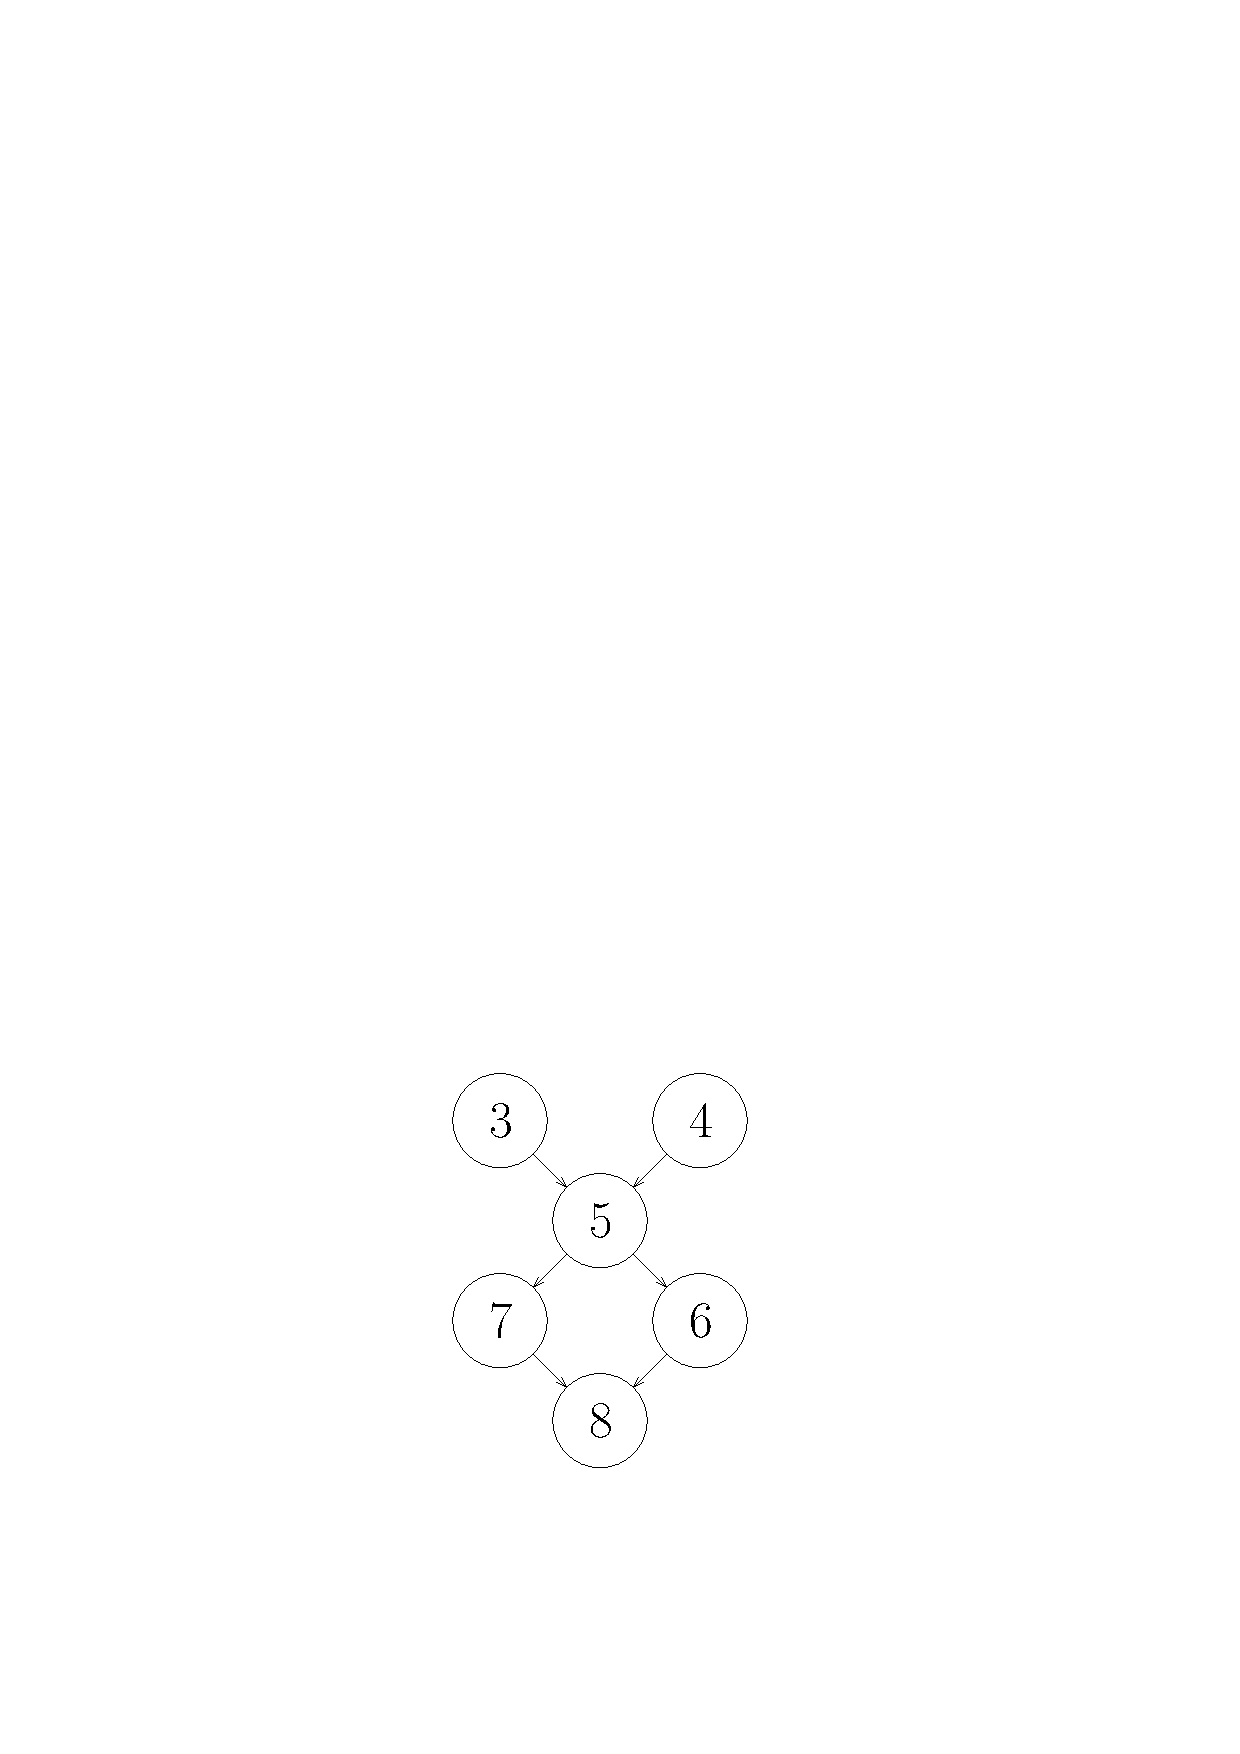
\includegraphics[scale=1]{Graphics/chapters}
\caption{A diagram depicting interrelations between the chapters.}\label{fig:chapters}
\end{figure}



